% Include at a fixed width: scaling DOWN would push the
% in-figure type below the 9pt floor the artwork guide sets.
\begin{figure}[t]
  \centering
  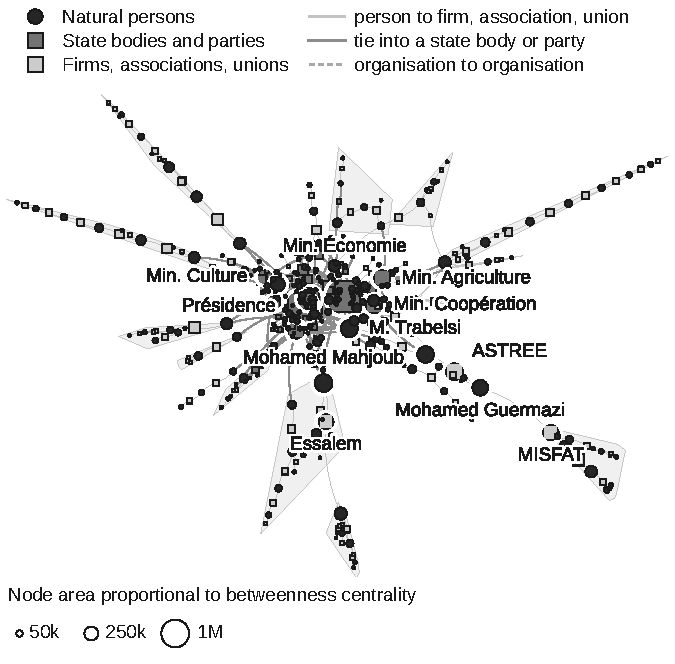
\includegraphics[width=4.5in]{fig16_brokerage_network_pre2011.pdf}
  \caption{\textbf{The brokerage core of the Tunisian elite network before 2011-01-14.}
  Node area is proportional to betweenness centrality. The 397
  entities shown, joined by 546 ties, are the giant
  component of the subgraph induced on the 400 highest
  betweenness entities, which together hold 91.7\% of
  all betweenness in the graph. Ties are those evidenced in the
  \emph{Journal Officiel} before 2011-01-14, the day Ben Ali left office:
  7,268 company board and officer ties and
  1,482 state offices, plus 119
  dated inter-organisational ties, over 9,734 entities in
  all. \textbf{This is a filter on source as well as on time.} Every
  gazette-evidenced tie in the dataset carries a date and every
  seed-derived tie carries none, so restricting to ties evidenced before a
  date necessarily drops the whole seed layer: shareholding, kinship,
  association and party membership are absent here, not because they did
  not exist before 2011, but because the roster that records them asserts
  present affiliations and is undated. Betweenness is recomputed on this
  graph and is not comparable with the pooled figure. The gazette also
  documents state appointments more completely than company officers,
  which will overstate the state's share relative to the private
  layer.
  The composition is 242 natural persons, 33 state bodies and
  parties, and 122 firms, associations and unions. The 11
  highest-brokerage entities are labelled. Abbreviations: Min. Économie, Ministère de l'Économie Nationale; Présidence, Présidence de la République; M. Trabelsi, Mohamed Trabelsi; ASTREE, Compagnie d'Assurances et de Réassurances ASTREE; Min. Coopération, Ministère de la Coopération Internationale et de l'Investissement Extérieur; Min. Agriculture, Ministère de l'Agriculture, de l'Environnement et des Ressources Hydrauliques; MISFAT, Société Tunisienne des Filtres MISFAT.}
  \label{fig:fig16_brokerage_network_pre2011}
\end{figure}

% ---------------------------------------------------------------------
% Accessibility description (APSR requires one; WCAG 2.1 AA)
% ---------------------------------------------------------------------
% A node-link diagram of 397 entities connected by
% 546 lines, drawn in greyscale. Circles are natural
% persons, squares are organisations; darker fills are state bodies and
% parties, lighter fills are firms, associations and unions. The area of
% each shape is proportional to its betweenness centrality, so the
% entities that lie on the most shortest paths appear largest. A small
% number of very large nodes, led by Min. Économie,
% sit at the centre of the diagram and connect several otherwise separate
% dense clusters of smaller nodes. A size key at the lower left gives
% reference areas in millions.
